% !TeX root = ../libro.tex
% !TeX encoding = utf8

\chapter{Rotación y campos magnéticos de intensidad constante}\label{ch:tercer-capitulo}

\section{Introducción}

El impacto de la rotación tanto en la PMS como en el agotamiento del Li para las estrellas de tipo solar ha sido ampliamente debatido en el pasado \cite{Pinsonneault1997,Jeffries2004,Somers2014} y revisado más recientemente sobre la base de la disponibilidad de medidas más precisas \cite{Bouvier2016}. Sin embargo, estos estudios previos se centraron principalmente en los efectos hidrostáticos y no consideraron la influencia de un acoplamiento entre el campo magnético estelar y su posible efecto de desacelaración. Se piensa que la AML tiene una influencia directa en los procesos de mezcla y que el transporte del momento podría producirse por una serie de mecanismos tales como: pérdida de masa, campos magnéticos y ondas gravitatorias (modos g). Respecto a estos dos últimos, las ondas gravitatorias \cite{Charbonnel2005, Pincon2016} y los campos magnéticos \cite{Eggenberger2009} tienen la propiedad de transmitir el momento angular (AM) de forma mucho más eficaz que inducir la mezcla \cite{Denissenkov2007}. Como consecuencia de este incremento en la eficiencia del transporte del AM, se reduce la cantidad de rotación diferencial entre las zonas radiativa y convectiva de la estrella (se fomenta una rotación de cuerpo sólido), así como las inestabilidades rotacionales inducidas. Además, también se originarían campos magnéticos en los límites entre estas zonas, en las llamadas tacoclinas \cite{Aschwanden2014, Guerrero2016}, que interaccionarían con las partículas del viento solar que se verían obligadas a rotar en sincronía con el campo magnético imperante y por tanto, frenarían la rotación estrella. Esto es lo que se conoce como el efecto de frenado magnético (Magnetic Braking, MB). \par

\begin{figure}
    \centering
    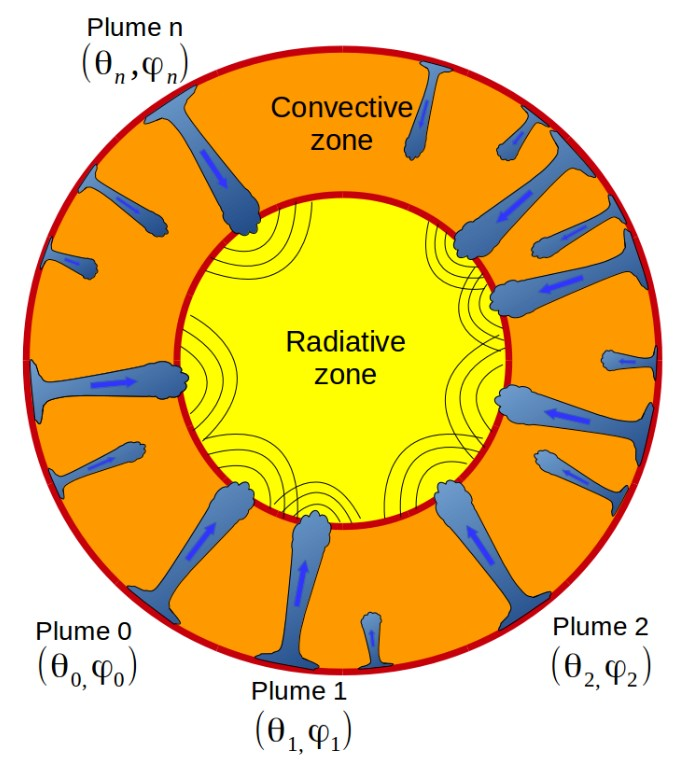
\includegraphics[width=0.5\textwidth]{img/tesis/gravitational_waves.jpg}
    \caption{Vista esquemática de la estrella. Los penachos convectivos se producen en las capas superiores de la estrella y se adentran en la región convectiva. Crecen por arrastre turbulento de materia en sus bordes y alcanzan la parte superior de la zona radiativa. Allí, cada una de ellas, caracterizada por su posición angular ($\theta_i$,$\phi_i$), libera una parte de su energía cinética y genera ondas internas que pueden propagarse hacia el centro. (Figura tomada de \cite{Pincon2016})}
    \label{fig:grav_waves}
\end{figure}

A día de hoy, los modelos estándar no son capaces de replicar de forma satisfactoria los valores observados de abundancia de Li en las superficies estelares con las predicciones que estos modelos arrojan. Esta falta de concordancia nos hace pensar que ciertos mecanismos físicos que influyen en la destrucción del Li están siendo modelizados de forma inadecuada o simplemente no se tienen en cuenta, como por ejemplo el frenado magnético. A la vista de estos hallazgos, parece evidente que aún quedan cuestiones abiertas por resolver sobre el tema de los procesos que participan, directa o indirectamente, en los mecanismos de mezcla que no están incorporados en los modelos estelares estándar. Por ello, es imprescindible una adecuada consideración de las interacciones entre rotación y campos magnéticos a la hora de estudiar la distribución del AM. \par

La abundancia de Li observada en la fotosfera de las estrellas es un indicador de su composición interior y de los procesos de mezclado que en su interior tienen lugar. Adicionalmente, estas abundancias (además de otras métricas) se utilizan para comprobar la validez de los modelos estelares. Para que esto sea posible hay que tomar como premisa inicial que la abundancia de Li generada en la nucleosíntesis asociada al Big Bang es conocida y este elemento solo se destruye a través de reacciones nucleares. A pesar de décadas de esfuerzos teóricos, se sigue sin encontrar una explicación coherente con los modelos para las discrepancias encontradas en las comparaciones sobre la abundancia de Li para estrellas pertenecientes a cúmulos de diferentes edades y que se encuentran en el mismo estado evolutivo, o bien en la PMS, o bien en MS. Los modelos no son capaces de explicar las abundancias detectadas en las etapas tardías de la MS \cite{Tschape2001}.\par

Es sabido que parte de la pérdida de Li se produce durante la PMS y que además ésta se acentúa según decrece la masa de la estrella y, a igualdad de masa, según aumenta la metalicidad de la misma. Para reproducir la dependencia entre la edad y masa de las estrellas con la merma de las concentraciones de Li, estos modelos necesitan de una combinación de procesos de mezclado cada vez más complejos, como overshooting, mezclado debido a procesos rotacionales o difusión microscópica.
Para las estrellas de tipo solar, nos encontramos con dos factores que tienen que ser explicados desde el punto de vista de la abundancia de Li:

\begin{enumerate}
    \item La deficiencia generalizada de Li en el Sol y en estrellas de tipo tardío presentes en cúmulos a diferentes edades.
    \item La gran dispersión en abundancia de Li que existe en estrellas con una determinada temperatura efectiva detectada en los cúmulos abiertos.
\end{enumerate}

Existen datos observacionales que sugieren que las estrellas que giran más rápido preservan el Li mejor que las que lo hacen más lentamente. Este hecho se puede deber a que por encima de cierto umbral de velocidad de rotación, ésta impide de manera drástica la penetración vertical de penachos generados por movimientos convectivos que, cuando están presentes, contribuyen a hacer más eficiente el proceso de destrucción de Li \cite{Baraffe2017}.\par

Adicionalmente y según el modelo estándar de nucleosíntesis para el Big Bang, la abundancia de Li original puede estimarse en 2.6 dex \cite{Spergel2003} pero la abundancia de litio detectadas en meteoritos se conoce que está en el orden A(Li) = [3.26-3.34] dex \cite{Randich2006, Grevesse2007}, lo que apunta hacia un enriquecimiento desde que se produjo el Big Bang. Por otro lado, la abundancia medida en las estrellas de tipo solar es del orden de ALi = 1.05 dex \cite{Grevesse2007}, lo que implica la existencia de procesos de destrucción del Li en su interior.  Esta discrepancia entre las abundancias medidas en meteoritos y en estrellas de tipo solar es lo que ha pasado a denominarse el “problema del litio”.\par

Continuando con la importancia del Li y teniendo en cuenta que tanto éste, como los demás elementos ligeros berilio y boro, se queman a temperaturas relativamente bajas en interiores estelares, tenemos que estos elementos sólo sobreviven en las capas más externas de una estrella, donde la temperatura es menor. Adicionalmente, su presencia es un trazador muy potente relacionado con los mecanismos de mezcla en funcionamiento en estructuras estelares, ya que nos puede aportar información acerca de qué tal eficientes son a la hora de transportar estos elementos a zonas más interiores donde serían destruidos.\par

\section{El Sol y la rotación}
Nuestro Sol, como estrella que es y como ocurre con el resto de los cuerpos celestes, gira en torno a su eje. El tiempo que tarda en completar una revolución completa sobre este es de aproximadamente 26 días. Decimos aproximadamente porque la duración del día solar es diferente dependiendo de la latitud que se tome como referencia. Si comparamos las velocidades de rotación solar y la terrestre con respecto al diámetro de los correspondiente cuerpos celestes, se obtiene que un punto situado sobre la superficie solar girar aproximadamente cuatro veces más rápido de lo que lo haría sobre la Tierra.

Esto ocurre porque, a diferencia de la Tierra, el Sol no es un cuerpo rígido. Por lo tanto, al estudiar la rotación del Sol, no se puede considerar como una estructura compacta. El Sol es en realidad una enorme esfera de plasma, más parecida a una enorme bola de gas que a una estructura sólida rígida.\par

Si tomamos como referencia medidas de la rotación solar a lo largo de un período largo de tiempo podemos observar que, dependiendo de la latitud que tomemos como referencia, la velocidad de rotación se va incrementando conforme la distancia al ecuador solar se reduce. Es decir, el Sol gira más rápidamente en el ecuador que en sus polos \ref{fig:rot_solar_vs_latitud}. Este comportamiento que se conoce como rotación diferencial fue descrito por Richard Carrington (1826-1875) tras analizar el movimiento de las manchas solares \cite{Carrington1863}. Carrington dedujo la siguiente ley empírica mediante donde $\Omega_*$ es la cantidad angular de la rotación diaria y $\phi$ es la latitud heliográfica, que corresponde a la latitud en la Tierra  \cite{Banisch2009}.\par

\begin{ceqn}
\begin{equation}
    \Omega_* = 14.4 - 2.8\sin^2\phi \label{eq:ang_rot_sun}
\end{equation}
\end{ceqn}

\begin{figure}
    \centering
    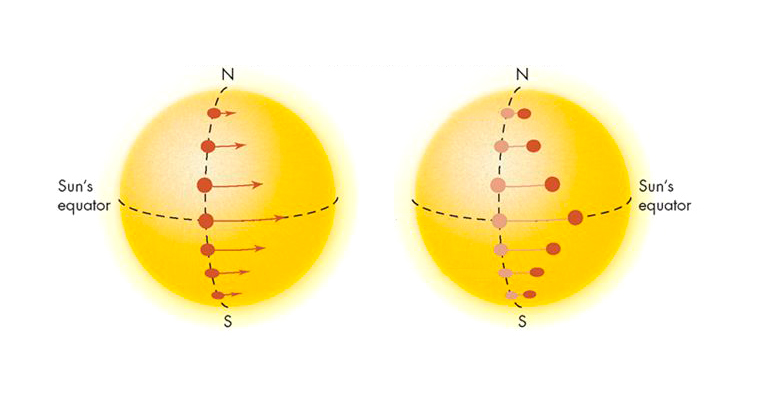
\includegraphics[width=0.8\textwidth]{img/tesis/sun_1.png}
    \caption{Rotación diferencial presente en el Sol. Tomando como referencia un meridiano solar y situando sobre este diferentes puntos de referencias a diferentes latitudes, se observa que la velocidad con la que estos giran es mayor a medida la distancia al ecuador solar disminuye. Crédito McGraw-Hill.}
    \label{fig:rot_solar_vs_latitud}
\end{figure}

El período de rotación $d_*$ en días se calcula como:

\begin{equation}\label{eq:dia_solar}
    d_* = \frac{360}{\Omega_*}
\end{equation}

En la región ecuatorial la rotación dura solo 25 días, mientras que en los polos el Sol gira más lentamente \ref{fig:ang_solar_vs_latitud}. Aquí el día solar tiene una duración aproximada de 30 días. A pesar de esta rotación diferencial entre regiones situadas en latitudes diferentes, no se produce un aplanamiento reseñable del disco solar ya que la velocidad de rotación es pequeña, de media 2km/s \cite{Gill2012}.\par

\begin{figure}
    \centering
    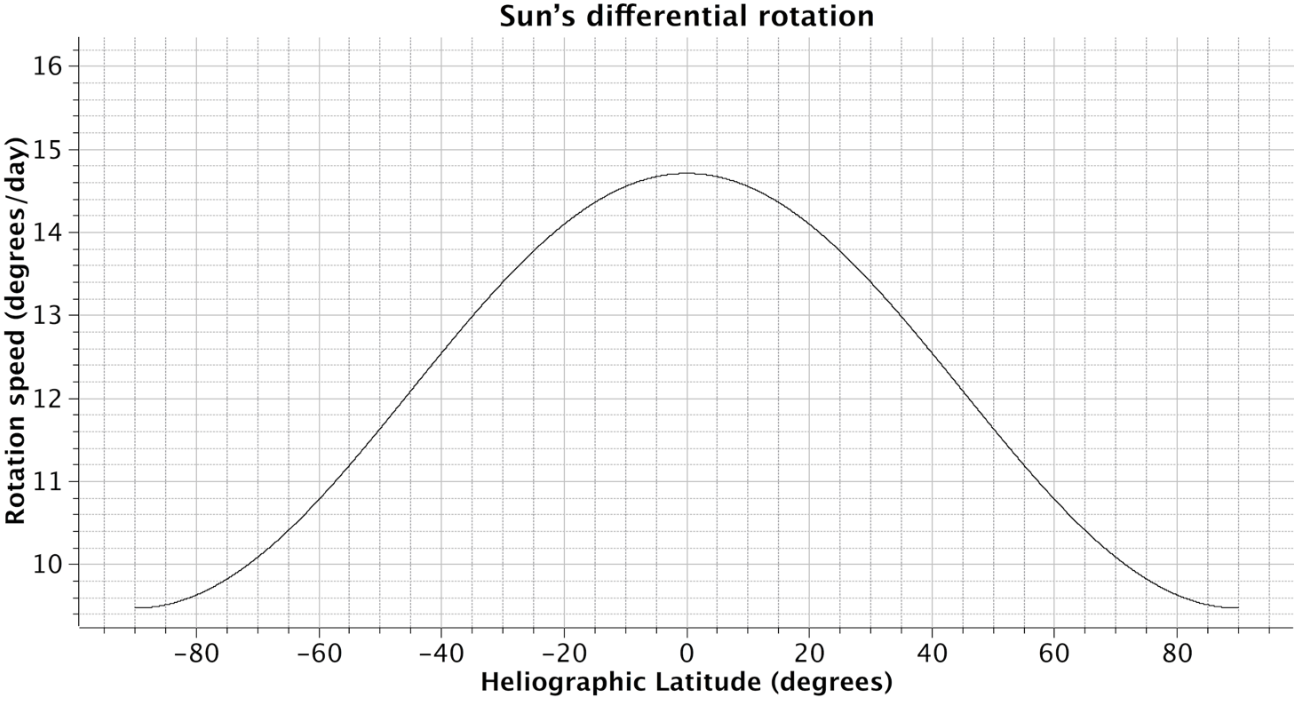
\includegraphics[width=1.0\textwidth]{img/tesis/sun_3.png}
    \caption{Valor predicho teóricamente para la velocidad de rotación del Sol en función de la latitud. Sobre el ecuador solar se obtiene la máxima velocidad angular y esta va disminuyendo a medida que aumenta la latitud. Crédito CESAR ESAC.}
    \label{fig:ang_solar_vs_latitud}
\end{figure}


\section{Efectos de los campos magnéticos}
Aún se desconoce el origen de los campos magnéticos en las estrellas. Los campos magnéticos organizados detectados en algunas estrellas O \cite{Wade2010} podrían ser campos fósiles \cite[ver][para más detalles ]{Dudorov2014}, o campos producidos mediante un mecanismo de dinamo \cite{Cantiello2009}. Además, la presencia de campos magnéticos con intensidades del orden de kG \cite{Hussain2014} ha sido una condición sine qua non para tratar ciertos datos observados en estrellas de tipo T Tauri en sistemas PMS jóvenes en acreción \cite{Johns-Krull2007}.\par

La masa de las estrellas juega un papel determinante en la existencia o no de una envoltura convectiva externa. A su vez, la presencia de esta región convectiva condiciona la evolución de los campos magnéticos. Las estrellas masivas no tienen zonas convectivas externas aunque pueden exponer un núcleo convectivo. En cambio, las estrellas menos masivas, como el Sol, tienen envolturas convectivas y un núcleo radiativo. En ambos tipos de estrellas se pueden generar fuertes campos magnéticos en la tacoclina pero con notables diferencias \cite[v.g.][para más detalles]{Chabrier2006,Charbonneau2010}.\par

En el Sol, la materia que lo compone se encuentra en su mayoría presente en forma de plasma. Es este estado, la envoltura electrónica se encuentra desacoplada del núcleo atómico y bajo ciertas condiciones físicas pueden moverse libremente, por lo que pueden poner en movimiento una carga electrónica. Bajo estas condiciones, la materia solar puede alcanzar la conductividad del cobre \cite{Banisch2009}.\par

\subsection{El mecanismo de dinamo}
Una dinamo es el proceso por el cual la energía mecánica se convierte
convierte en energía electromagnética por inducción. La energía mecánica se debe al movimiento de los fluidos y la energía electromagnética resultante produce los campos magnéticos observados. Para que una estrella tenga un campo magnético generado por dinamo, debe contener una región fluida conductora de electricidad que experimente movimientos para generar inducción. Sin embargo, existen otras condiciones necesarias para el vigor y la morfología de los movimientos que se derivan del hecho de que el campo magnético no debe decaer debido a la disipación óhmica. La necesidad básica para mantener un mecanismo de dinamo es una región fluida eléctricamente conductora en el interior de la estrella.

El Sol se rige por un fuerte campo magnético que se genera con una intensidad de campo magnético de B z 10 5 G \cite{Aschwanden2014} en la tacoclina, la delgada capa de cizalla intercalada entre la zona radiativa y la convectiva. Los tubos de flujo magnético flotante se elevan a través de la zona de convección (debido a la inestabilidad convectiva que obedece a la ley de Schwarz).
que obedece al criterio de Schwarzschild) y emergen en la superficie solar en las regiones activas, donde forman manchas solares con intensidades de campo magnético de B z 10 3 G y bucles coronales con intensidades de campo de B z 10 2 G en los puntos de apoyo fotosféricos, y de B z 10 G en las mayores alturas coronales. Se cree que la rotación diferencial en la superficie solar enrolla el campo magnético superficial, que se fragmenta bajo la tensión magnética, circula meridionalmente hacia los polos y se reorienta desde el estado de tensión toroidal (con líneas de campo orientadas en dirección este-oeste) en el máximo solar a un campo dipolar poloidal (que conecta el polo norte con el polo sur) en el mínimo solar.
mínimo solar.

\subsection{Campos magnéticos internos}
Nuestro Sol es una estrella activa en lo que se refiere al campo magnético. Según los modelos teóricos este campo magnético es generado por una dinamo en la tacoclina y con una intensidad en torno a $B\approx10^{5}\,\Gauss$ \cite{Maeder2003a,Dudorov2014}. En el momento de su generación, las líneas de ese campo magnético tendrán una orientación poloidal y se verán afectadas por la rotación diferencial y obligadas a adoptar una tipología toroidal (el efecto $\omega$). Por otro lado, también puede darse el caso contrario, partiendo de un campo magnético toroidal obtener una configuración poloidal. Esto sería posible gracias a los movimientos convectivos de material que se producen en el CZ de la estrella y suponer que este material se comporta como un conductor perfecto. Esta segunda condición permite suponer que las líneas de campo magnético están "congeladas" en el fluido conductor y por tanto deben moverse solidariamente con él (efecto $\alpha$) \cite{Stanley2014}.\par

\begin{figure}
    \centering
    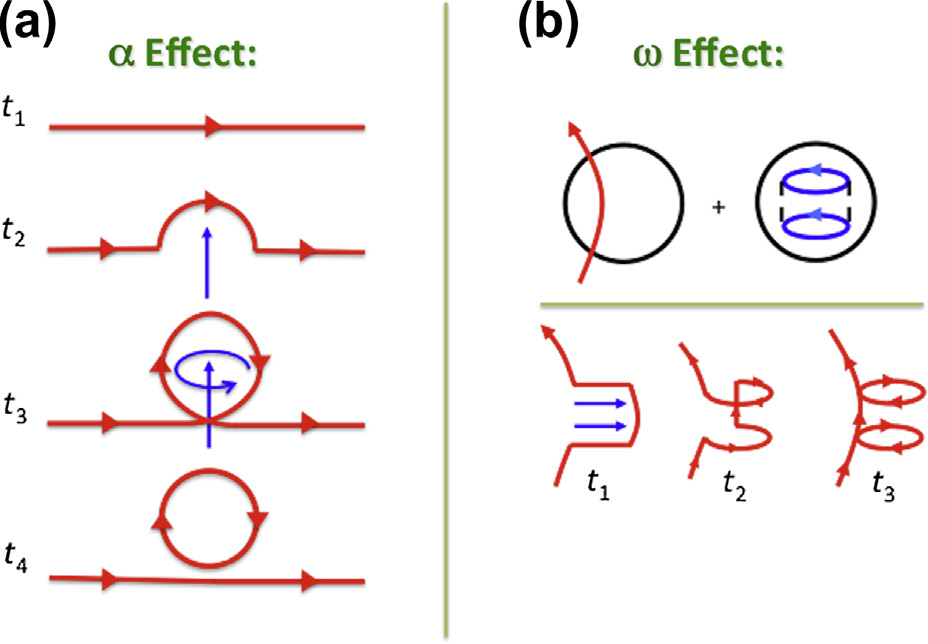
\includegraphics[width=0.6\textwidth]{img/tesis/alpha_omega_effect.png}
    \caption{Esquema de los mecanismos canónicos de generación de dinamo. Las líneas de campo magnético están en rojo y los campos de velocidad en azul. \textbf{(a)} En el efecto, un flujo helicoidal estira ($t_2$) y luego retuerce ($t_3$) el campo magnético. Una pequeña cantidad de difusión en el punto de torsión ($t_4$) puede generar un bucle de campo magnético ortogonal al campo original. \textbf{(b)} En el efecto $\omega$, una rotación diferencial a gran escala afecta una línea de campo poloidal y la estira en dirección zonal ($t_1$ - $t_3$) generando bucles magnéticos toroidales a partir de la línea de campo poloidal. El círculo negro indica el límite exterior de la región de la dinamo. \cite{Stanley2014}}
    \label{fig:alpha_omega_effect}
\end{figure}


\subsection{Campos magnéticos superficiales} \label{surf_mf}
La intensidad del campo magnético medida en la superficie del Sol es de aproximadamente $B\approx1\,\Gauss$ \cite{Weber1967,DAntona2000,Morin2012}, el doble del valor del de la Tierra. Además su topología es variada y compleja. El modelo de dinamo establece que el campo magnético producido en el interior de la estrella alcanza la superficie con la ayuda de procesos convectivos que tienen lugar en la CZ y da lugar a regiones magnéticamente activas en la superficie solar. Además, las estrellas en rotación que exponen una CZ exterior significativa pueden producir campos magnéticos superficiales a través de un mecanismo de dinamo \cite[v.g.][]{Brandenburg2004,Charbonneau2010,Brun2017}. Sea cual sea el origen de los campos magnéticos superficiales, se predice un acoplamiento con el viento estelar, provocando así una pérdida de masa y, si ésta es lo suficientemente fuerte, produzcan MB \cite[v.g.][]{UdDoula2002,Ud-Doula2007,Ud-Doula2008,Meynet2010}.\par


\section{Efectos del frenado magnético - Parte I}
En su enfoque más aceptado, el MB está vinculado al trabajo de Skumanich \cite{Skumanich1972} en el que desarrolla una ley empírica de su evolución en paralelo a la edad de la estrella. Para calibrar esta ley, Skumanich se basó en datos obtenidos de estrellas de tipo G encontradas en la MS. La influencia del MB en la evolución de la estrella está estrechamente relacionada con el transporte del AM. Según \cite{Meynet2010}, se distinguen dos mecanismos principales atendiendo a cómo se produce el transporte del AM:

\begin{enumerate}
    \item Rotación diferencial: el transporte de AM es impulsado por corrientes meridionales e inestabilidades de cizalla.
    \item Rotación de cuerpo sólido: cuando el transporte de AM es muy eficiente, la rotación de cuerpo sólido se mantiene durante toda la MS.
\end{enumerate}

El AML causado por MB depende directamente de la cantidad de masa perdida por la estrella debido a los vientos estelares. El coeficiente de pérdida de masa estimado para una estrella de tipo solar, aproximadamente $10^{-14}\msun \; yr^{-1}$ \cite{Noerdlinger2008}, y el AML resultante derivado de ese valor pueden considerarse relativamente modesto como para influir decisivamente en la evolución de la estrella. Además, el efecto combinado de los movimientos convectivos y la rotación diferencial conducen a la generación de campos magnéticos. Esos campos magnéticos acaban alcanzando la superficie de la estrella, de modo que el AML puede incrementarse en varios órdenes de magnitud \cite{Langer2012}. Ese incremento es consecuencia del campo magnético que obliga a las partículas ionizadas del viento estelar a girar con la misma velocidad angular, vientos que se extienden una distancia varias veces superior al radio de la estrella \cite[ver][para más detalles]{UdDoula2002,Ud-Doula2007,Ud-Doula2008}.

Además, a lo largo de la evolución de la estrella, parámetros directamente observables como su velocidad de rotación, temperatura efectiva, gravedad superficial o abundancia de elementos químicos sufren variaciones. Estos parámetros influyen, directa o indirectamente, en la pérdida de momento angular causada por el campo magnético de la estrella.\par


\subsection{Formalismo de frenado magnético de intesidad fija} \label{mod_mb}
Comenzamos enumerando los aspectos más relevantes y las suposiciones realizadas en la modelización de la evolución de la rotación, el frenado magnético y el momento angular en MESA. Estos serán considerados para el cálculo del AML como resultado del par aplicado por un viento estelar acoplado magnéticamente.\par 

En presencia de pérdida de masa, el material del viento estelar elimina el AM, lo que provoca un efecto de giro a la baja. Esto es muy importante, por ejemplo, en las estrellas masivas, que se sabe que rotan rápidamente y tienen fuertes vientos estelares. También se ha observado que las estrellas de masa intermedia fuertemente magnéticas suelen tener tasas de rotación mucho más lentas que otras estrellas de su población parental \cite{Mathys2006}. En esas estrellas, la presencia de dicho campo magnético interactuará con la pérdida de masa y el radio Alfv'{e}n ($R_{A}$) juega un papel importante en esta interacción.\par

En el resto de este trabajo, describimos dos enfoques semi-empíricos para el cálculo del AML como resultado del par aplicado por un viento estelar acoplado magnéticamente. Esto se ha implementado como una extensión del código de evolución estelar Modules for Experiments in Stellar Astrophysics \cite[MESA; ][]{Paxton2011, Paxton2013,Paxton2015, Paxton2018, Paxton2019}.

\subsubsection{Frenado magnético de intesidad fija según Ud-Doula \& Owocki (2002)}
Un parámetro relevante para caracterizar la influencia de un campo magnético dado sobre el viento estelar es el denominado parámetro magnético de confinamiento del viento ($\eta_*$). Representa una relación energética (Ec.~\ref{eq:wind_conf}) y define un parámetro característico de la eficacia relativa de los campos magnéticos para circunscribir y/o canalizar el flujo de salida del viento \cite{UdDoula2002}.\par

\begin{ceqn}
\begin{equation}
    \eta_* = \frac{B^{2}/8 \pi}{3} \label{eq:wind_conf2}
\end{equation}
\end{ceqn}


\begin{ceqn}
\begin{equation}
    \eta_* = \frac{B^{2}/8\pi}{\rho\nu^2/2} \label{eq:wind_conf}
\end{equation}
\end{ceqn}

donde $B^{2}/8\pi$ es la densidad de energía del campo magnético, $\frac{1}{2}\rho\nu^{2}$ la densidad de energía cinética, $B$ la intensidad del campo magnético, $\rho$ la densidad de masa, y $\nu$ la velocidad del viento estelar.\par

Haciendo uso de $\eta_*$, el $R_{A}$ se define como el punto en el que se equilibran la densidad de energía del campo magnético, marcada $B$, y la densidad de energía cinética, definida por $\rho$ y $(\nu)$. Es decir, donde el coeficiente entre ambos es igual a 1. En caso de que $R_{A}$ sea mayor que el radio de la estrella, entonces el flujo del viento tendrá que seguir el campo magnético. Como consecuencia, el material saldrá de la superficie estelar con un AM específico mayor, ya que el radio de co-rotación ha aumentado y corresponderá aproximadamente al $R_{A}$. Este efecto se conoce como MB.\par

Las estrellas con masas iniciales similares pero diferentes relaciones de pérdida de masa ($\Dot{M}$) acabarán evolucionando de forma muy diferente. Las partículas ionizadas transportadas por el viento solar no sólo contribuyen a la pérdida de masa, sino también a la pérdida de energía cinética que se deposita en el medio interestelar. Dada una estrella con un viento esféricamente simétrico, $\Dot{M}$ se caracteriza por la siguiente expresión:

\begin{ceqn}
\begin{equation}
    \Dot{M} = 4\pi r^2\rho\nu \label{eq:mass_loss}
\end{equation}
\end{ceqn}

Usando (\ref{eq:wind_conf}) and (\ref{eq:mass_loss}), $\eta_*$ puede ser aproximado por: 
\begin{ceqn}
\begin{equation}
    \eta_* = \frac{B^{2}r^{2}}{\Dot{M}\nu} \label{eq:wind_conf2}
\end{equation}
\end{ceqn}

\begin{ceqn}
\begin{align}
    \Dot{M} &= 4\pi r^2\rho\nu \label{eq:mass_loss}\\
    K_e &= 0.5\Dot{M}\nu_{esc}
\end{align}
\end{ceqn}


\begin{ceqn}
\begin{equation}
    \eta_* = \frac{B^{2}r^{2}}{\Dot{M}\nu} \label{eq:wind_conf2}
\end{equation}
\end{ceqn}

\begin{equation}\label{eq:identidad-pitagorica2}
  \cos^2 x + \sin^2 x = 1.
\end{equation}

A su vez, de las características observables del viento solar, nos importan especialmente los parámetros relacionados con la cantidad de masa que es capaz de arrancar de las capas externas de la estrella en un intervalo de tiempo dado, y la velocidad que alcanza el propio viento medida a gran distancia de la estrella, la velocidad terminal ($\nu_\infty$). En general, un flujo de salida canalizado magnéticamente tendrá una geometría de corriente compleja pero, por conveniencia, la Ec.~\ref{eq:mass_loss} simplemente caracteriza la fuerza del viento en términos de una tasa de pérdida de masa distribuida simétricamente sobre una esfera. $\nu$ puede caracterizarse por la variación radial de la velocidad del flujo saliente en términos de la ley de velocidad (Ec.~\ref{eq:vel_law}), donde $r$ representa la distancia desde el centro de la estrella hasta el punto donde se va a medir la velocidad, y $R_*$ es el radio de la estrella:\par

\begin{ceqn}
\begin{equation}
    \nu(r) = \nu_\infty (1-R_*/r) \label{eq:vel_law}
\end{equation}
\end{ceqn}
donde $\nu_\infty$ es la velocidad terminal del viento definida como la velocidad que alcanza el viento, la materia que fluye a gran distancia de la estrella central, donde ya no es acelerada por la fuerza impulsora del viento pero su desaceleración debida a la interacción con el medio interestelar (ISM) es despreciable \cite{Niedzielski2002}.\par

Los vientos impulsados por líneas de las estrellas OB masivas tienen velocidades terminales que son directamente proporcionales a la velocidad de escape fotosférica \cite{Lamers2000} según:\par

\begin{ceqn}
\begin{align}
    \nu_\infty &\simeq 1.92 \;\nu_{\textrm{esc}} \label{eq:vinf}\\
    \nu_{\textrm{esc}} &= \sqrt{\frac{2\,G\,\mstar}{\rstar}} \label{eq:vesc}
\end{align}
\end{ceqn}

donde la Ec.~\ref{eq:vesc} describe la velocidad de escape newtoniana desde la superficie estelar, donde $G$ es la constante gravitatoria, ${\rstar}$ el radio, y ${\mstar}$ la masa de la estrella.

Haciendo uso de (\ref{eq:vesc}), $\nu_\infty$ puede reformularse como:
\begin{ceqn}
\begin{equation}
    \nu_\infty \simeq 1.92 \; x \; 618 \; \Bigg(\sqrt{\frac{\rsun}{\rstar}\frac{\mstar}{\msun}} \;\Bigg) \label{eq:vinf}
\end{equation}
\end{ceqn}
donde ${\rsun}$ es el radio, y ${\msun}$ la masa del Sol.


Dado que la versión de MESA utilizada en este trabajo no incluye el tratamiento de los campos magnéticos superficiales (sí tiene en cuenta el transporte por campos magnéticos internos de momento angular y elementos químicos) y, por tanto, tampoco los efectos de frenado magnético, es necesario extender el simulador para incluir este fenómeno. En la presente tesis hemos seguido el trabajo teórico sobre el AM en el Sol realizado por \cite{Weber1967}, haciendo uso de la Ec.~ \ref{eq:j_dot} para el cálculo del AML.\par

Se ha observado que las estrellas de masa intermedia fuertemente magnéticas suelen tener tasas de rotación mucho más lentas que otras estrellas de su población parental \cite{Mathys2006}. En esas estrellas, los campos magnéticos interactúan con la pérdida de masa, donde el radio Alfv'{e}n ($R_{A}$) juega un papel importante. Haciendo uso de $\eta_*$ (Ec. \ref{eq:wind_conf}), $R_{A}$ se define como el punto en el que la densidad de energía del campo magnético y la densidad de energía cinética se equilibran. En caso de que $R_{A}$ sea mayor que el radio estelar, entonces el flujo del viento tendrá que seguir el campo magnético. Como consecuencia, el material abandona la superficie estelar con un AM específico mayor, ya que el radio de co-rotación ha aumentado y corresponde aproximadamente a $R_{A}$. Siguiendo a \cite{Weber1967} el AML puede calcularse mediante:

\begin{ceqn}
\begin{equation}
 \Dot{J} = \frac{2}{3} \Dot{M}\Omega R^{2}_{A} \label{eq:j_dot}
\end{equation}
\end{ceqn}

donde $\Dot{M}$ es la tasa de pérdida de masa, $\Omega$ la velocidad angular en la superficie de la estrella y $R_A$ el radio Alfv\'{e}n. \par

La expresión anterior se puede reescribir según \cite{Ud-Doula2008} de modo que dependa de $\eta_*$ en lugar de $R_A$ como sigue:

\begin{ceqn}
\begin{equation}
 \Dot{J} = \frac{2}{3} \Dot{M}\Omega R^{2}_{*}\eta_* \label{eq:j_dot_mesa}
\end{equation}

\end{ceqn}
que es una expresión más conveniente para ser implementada en MESA porque se basa en valores directamente expuestos durante las simulaciones.



\section{Efectos de la distrubución de AML}
\subsection{Formalismo para la distribución de AML} \label{mod_aml}
Como expresa la Eq.~\ref{eq:mb_torque}, la cantidad de AML depende de $\ralfven$, $\Omega$ y $\Dot{M}$. Para valores grandes de $\ralfven$, la estrella sufre una desaceleración significativa. El valor de $\ralfven$ depende de los siguientes parámetros variables: intensidad del campo magnético ($B$), $\teff$ y $\Omega$. Con respecto a $\Dot{M}$ y como se indica en la tabla \ref{tab:phy_mesa}, para calcular la pérdida de masa se utilizó la fórmula empírica desarrollada por Reimers \cite{Reimers1975} para estrellas en la rama gigante asintótica (AGB). Para una estrella de tipo solar el $\Dot{M}$ durante la EM es relativamente pequeño, alrededor de $10^{-14}\msun \, yr^{-1}$ \cite{Noerdlinger2008}. \par

MESA asigna un valor $\Omega$ para cada celda $k$ ($\Omega_k$) que se ajusta para que el momento angular resultante se conserve tras calcular la nueva masa de la celda $k$ ($m_k$) y su distancia al centro de la estrella ($r_k$). A continuación, se asigna un valor de AM a cada celda $k$ ($J_k$). En este punto, nuestro MB se activa, modificando $J_k$. Para ello, se proporciona una contribución adicional ($\Dot{J}_{k}$). Esta contribución es el resultado del par externo ejercido por el campo magnético una vez que se ha distribuido entre las diferentes capas que componen la CZ según dicta la Eq.~\ref{eq:k_jdot}:\par

\begin{ceqn}
	\begin{align}
		\Dot{J}_{k} &= \Dot{J}_*\;\frac{m^{}_{k} r^2_{k}}{m^{}_* r_*^2} \label{eq:k_jdot}
	\end{align}
\end{ceqn}

La distribución se realiza en dos iteraciones. En la primera iteración, a cada celda $k$ se le asigna la cantidad máxima de $\Dot{J}_{k}$ que puede acomodar en el paso de tiempo establecido por la simulación. Las cantidades de $\Dot{J}_{k}$ no acomodadas por las celdas se acumulan como momento angular residual ($\jres$). En una segunda pasada, el valor $\jres$ residual acumulado recogido en la iteración anterior se redistribuye entre aquellas celdas que pueden acomodar más par. De esta forma conseguimos conservar el momento angular.\par


\section{Extendiendo MESA - Parte II}

\subsection{Rutina de frenado magnético de intensidad constante}
EXPLICAR QUE SUSTITUIMOS LA RUTINA POR DEFECTO CON LA NUESTRA
\begin{lstlisting}[language=Fortran, caption={Rutina de par de torsión.}, label={lst:jdot_cantiello}]
	real function calculate_jdot_rate_cantiello(s, bf_star) result(new_j_dot)
	use const_def
	type (star_info), pointer, intent(in) :: s
	real(dp), intent(in) :: bf_star
	
	real(dp) :: r_st, m_st, i_st, alfven_r
	real(dp) :: omega_surf, m_dot, eta_surf, v_inf, v_esc
	
	!Star data
	r_st = s% r(1)
	m_st = s% m(1)
	omega_surf = s% omega(1)
	!omega_surf = s% omega_avg_surf
	
	! escape and infinite velocities
	! 100000 transform from km/s to cm/s
	v_esc = (618 * ((Rsun/r_st)*(m_st/Msun))**0.5) * 100000
	v_inf = 1.92 * v_esc
	
	!m_dot = s% star_mdot !This gives the mass loss rate in Mstar/year
	m_dot = s% mstar_dot !This in g/s
	
	eta_surf = ((r_st * bf_star)**2)/(abs(m_dot) * v_inf)
	
	!Formula 2.3 Cantiello's MESA assigment
	new_j_dot = two_thirds * m_dot * omega_surf * (r_st**2) * eta_surf
	end function
\end{lstlisting}


\subsection{Rutina de distribución de pérdida de momento angular}
EXPLICAR QUE LOS DOS TIPOS DE RUTINAS: INTESIDAD FIJA, INTENSIDAD VARIABLE
\begin{lstlisting}[language=Fortran, caption={Rutina de distribución de pérdida de momento angular.}, label={lst:dis_jdot}]
	subroutine distribute_j_dot(s, total_j_dot, sz_info, mb_jdot_list)
	type (star_info), pointer, intent(in) :: s
	real(dp), intent(in) :: total_j_dot
	type (star_zone_info), pointer, intent(in) :: sz_info
	real(dp), dimension(:), pointer, intent(out) :: mb_jdot_list
	integer :: k
	real(dp) :: sum_jdot, dm_jdot, dm_bar_jdot, factor
	
	!By default, no lost of angular moment
	mb_jdot_list(:) = 0.0
	
	do k = sz_info% top_zone, sz_info% bot_zone, 1
	!Here the jdot distribution strategy is defined
	!Simple rule of three distribution loss of angular momentum based on the 
	!angular momentum of the zone vs total angular momentum of the convective zone
	
	!IMPORTANT: Don't forget to divide by dm(k) in order to get an "specific" jdot
	mb_jdot_list(k) = ((s% dm(k) * s% r(k)**2 * total_j_dot) / &
	(sz_info% d_mass * sz_info% d_radius**2)) / s% dm(k)
	
	end do
	end subroutine distribute_j_dot
	
\end{lstlisting}





\endinput
%--------------------------------------------------------------------
% FIN DEL CAPÍTULO. 
%--------------------------------------------------------------------
